\documentclass[11pt]{scrartcl}
\usepackage{ebb}



\title {Doble Conteo}
\subtitle {Entrenamientos Nacionales Centros Pagmos}

\author{Emmanuel Buenrostro}

\begin{document}
\maketitle

\section{Teoria}
\begin{itemize}
    \item Contar de dos formas distintas
    \item Ejemplo 1 Pascal 
    \item Ejemplo 2
    \item Hacer tablas, ejemplo 3
\end{itemize}

\section{Problemas }
\epigraph{The world has ended for me many times, and yet tomorrow still comes.}{Amber Glenn}

\subsection{Nivel I}


\begin{problem} %[IMO HK Prelim 2003]
    Quince estudiantes se inscriben en un curso de verano. Cada dia, tres estudiantes estan de guardia despues de clases para limpiar el salon. Al terminar el curso, se observo que cada par de estudiantes ha estado de guardia junto exactamente una vez. ¿Cuantos dias dura el curso?
\end{problem}

\begin{problem} %[Handshake lemma]
    Demuestra que en un grafo, la suma de los grados de cada vertice es igual a el doble de la cantidad de aristas.
\end{problem}

\begin{problem}
    Demuestra que 
    \[\binom{n}{0}+\binom{n}{1}+\ldots+\binom{n}{n}=2^n\]
\end{problem}

\begin{problem} %[Palo de Hockey]
    Sean $k$ y $n$ enteros no negativos, demuestra que  
    \[\binom{n+1}{k+1}=\binom{k}{k}+\binom{k+1}{k}+\binom{k+2}{k}+\ldots +\binom{n}{k}\]
\end{problem}

\begin{problem} %[PAGMO 2022/1]
    
    Leticia tiene un tablero de $9\times 9$ casillas. Se dice que dos casillas son amigas si comparten un lado o si están en una misma columna, pero en extremos opuestos, o si están en una misma fila, pero en extremos opuestos. De esta forma, cada casilla tiene exactamente $4$ casillas amigas. Leticia va a pintar cada casilla de uno de tres colores: verde, azul o rojo. Una vez que todas las casillas estñen pintadas, en cada casilla se va a escribir un número, siguiendo las siguientes reglas:
 \begin{itemize} 
 \item  Si la casilla es verde, se escribe la cantidad de casillas rojas amigas más dos veces la cantidad de casillas azules amigas.
 \item  Si la casilla es roja, se escribe la cantidad de casillas azules amigas más dos veces la cantidad de casillas verdes amigas.
 \item  Si la casilla es azul, se escribe la cantidad de casillas verdes amigas más dos veces la cantidad de casillas rojas amigas.
 \end{itemize} 
Encuentra el máximo valor posible de la suma de los números asignados a las casillas que Leticia puede obtener, sabiendo que ella puede escoger la coloración de las casillas del tablero.

    
\end{problem}

\subsection{Nivel II}

\begin{problem} %[IMC 2002]
    Doscientos estudiantes participaron en un concurso de matematicas. Tenian seis problemas para resolver. Se sabe que cada problema fue resuelto correctamente por al menos 120 participantes. Demuestra que deben existir dos participantes tales que cada problema fue resuelto por al menos uno de estos dos estudiantes.
\end{problem}

\begin{problem} %[CHKMO 2007]
    En una escuela hay $2007$ estudiantes hombres y $2007$ estudiantes mujeres. Cada estudiante se une a no mas de $100$ clubes en la escuela. Se sabe que cualquier par de estudiantes de generos opuestos ha pertenecido al menos a un club en comun. Demuestra que existe un club con al menos $11$ miembros hombres y $11$ miembros mujeres.
\end{problem}

\begin{problem}
    Demuestra que 
    \[1\binom{n}{1}^2+2\binom{n}{2}^2+\ldots+n\binom{n}{n}^2=n\binom{2n-1}{n}\]
\end{problem}

\begin{problem}
    Hay $10001$ estudiantes en una universidad. Algunos estudiantes se juntan para formar varios clubes (un estudiante puede pertenecer a distintos clubes). Algunos clubes se juntan para formar varias sociedades (un club puede pertenecer a distintas sociedades). En total hay $k$ sociedades. Supongamos que se cumplen las siguientes condiciones:
\begin{enumerate}
    \item Cada par de estudiantes esta en exactamente un club.

\item  Para cada estudiante y cada sociedad, el estudiante esta en exactamente un club de esa sociedad.

\item  Cada club tiene un numero impar de estudiantes. Ademas, un club con ${2m+1}$ estudiantes ($m$ es un entero positivo) pertenece exactamente a $m$ sociedades.
\end{enumerate}
Encuentra todos los posibles valores de $k$.
\end{problem}

\begin{problem} %[IMO 1987]
    Sea $p(n,k)$ el numero de permutaciones del conjunto $\{1,2,\dots,n\}$, $n\ge 1$, que tienen exactamente $k$ puntos fijos. Demuestra que
\[
\sum_{k=0}^{n} k\cdot p(n,k)=n!.
\]
\end{problem}

\subsection{Nivel III}

\begin{problem} %[OMM 2021/3]
    
    Sean $m,n\geq 2$ dos enteros. En una cuadrícula de $m\times n$, una hormiga empieza en el cuadrito inferior izquierdo y quiere caminar al camino superior derecho. Cada paso que da la hormiga debe ser a un cuadrito adyacente, y de acuerdo a las siguientes posibilidades: $\uparrow$, $\rightarrow$ y $\nearrow$. Sin embargo, un malvado mago ha dejado caer lava desde arriba de la cuadrícula y ha destruido algunos cuadritos, de forma tal que:
 \begin{itemize} 
 \item Si un cuadrito está destruido, entonces todos los cuadritos superiores a él también también están destruidos.

 \item El número de cuadritos destruidos es mayor o igual a $0$.

 \item Quedan suficientes cuadritos sin destruir para que la hormiga pueda llegar a la meta. 
 \end{itemize} 
Sea $P$ el número de caminos de longitud par que puede seguir la hormiga. Sea $I$ el número de caminos de longitud impar que puede seguir la hormiga. Encuentra todos los posibles valores de $P-I$.
    \begin{center}
        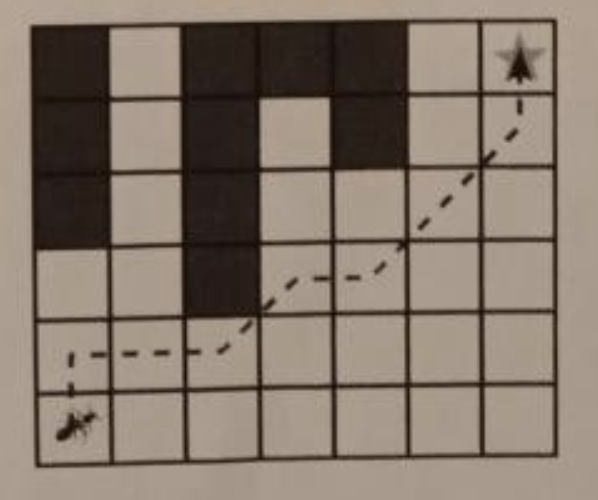
\includegraphics[scale=0.2]{21OMM3.png}
    \end{center}
\end{problem}

\begin{problem} %[IMO 1989/3]
    Sean $n$ y $k$ enteros positivos y sea $S$ un conjunto de $n$ puntos en el plano tal que

(a) no hay tres puntos de $S$ colineales, y

(b) para todo punto $P$ de $S$ hay al menos $k$ puntos de $S$ que estan a la misma distancia de $P$.

Demuestra que
$$
k < \frac{1}{2} + \sqrt{2\cdot n}.
$$
\end{problem}

\begin{problem} %[IMO 1998/2]
    En un concurso, hay $m$ candidatos y $n$ jueces, donde $n\ge 3$ es un entero impar. Cada candidato es evaluado por cada juez como aprobado o reprobado. Supongamos que cada par de jueces coincide en a lo mas $k$ candidatos. Demuestra que
\[
\frac{k}{m} \ge \frac{n-1}{2n}.
\]
\end{problem}

\begin{problem} %[Ibero 2001/3]
    
    Sean $S$ un conjunto de $n$ elementos y $S_1, S_2, \cdots , S_k$ subconjuntos de $S$ ($k \geq 2$), tales que cada uno de ellos tiene por lo menos $r$ elementos. \newline 
Demostrar que existen $i$ y $j$, con $1 \leq i < j \leq k$ tales que la cantidad de elementos comunes de $S_i$ y $S_j$ es mayor o igual que
\[ r - \frac{nk}{4(k-1)} \]

    
\end{problem}

\begin{problem} %[Kurschak 2019/2]
    ncuentra todas las familias $\mathcal{F}$ de subconjuntos de $[n]$ tales que, para cualquier subconjunto no vacio $X\subseteq [n]$, exactamente la mitad de los elementos $A\in \mathcal{F}$ satisfacen que $|A\cap X|$ es par.
\end{problem}

\end{document}